% CVPR 2022 Paper Template
% based on the CVPR template provided by Ming-Ming Cheng (https://github.com/MCG-NKU/CVPR_Template)
% modified and extended by Stefan Roth (stefan.roth@NOSPAMtu-darmstadt.de)

\documentclass[10pt,twocolumn,letterpaper]{article}

%%%%%%%%% PAPER TYPE  - PLEASE UPDATE FOR FINAL VERSION
% \usepackage[review]{cvpr}      % To produce the REVIEW version
\usepackage{cvpr}              % To produce the CAMERA-READY version
%\usepackage[pagenumbers]{cvpr} % To force page numbers, e.g. for an arXiv version

% Include other packages here, before hyperref.
\usepackage{graphicx}
\usepackage{amsmath}
\usepackage{amssymb}
\usepackage{booktabs}


% It is strongly recommended to use hyperref, especially for the review version.
% hyperref with option pagebackref eases the reviewers' job.
% Please disable hyperref *only* if you encounter grave issues, e.g. with the
% file validation for the camera-ready version.
%
% If you comment hyperref and then uncomment it, you should delete
% ReviewTempalte.aux before re-running LaTeX.
% (Or just hit 'q' on the first LaTeX run, let it finish, and you
%  should be clear).
\usepackage[pagebackref,breaklinks,colorlinks]{hyperref}


% Support for easy cross-referencing
\usepackage[capitalize]{cleveref}
\crefname{section}{Sec.}{Secs.}
\Crefname{section}{Section}{Sections}
\Crefname{table}{Table}{Tables}
\crefname{table}{Tab.}{Tabs.}


%%%%%%%%% PAPER ID  - PLEASE UPDATE
\def\cvprPaperID{*****} % *** Enter the CVPR Paper ID here
\def\confName{CVPR}
\def\confYear{2022}


\begin{document}

%%%%%%%%% TITLE - PLEASE UPDATE
\title{EEEM066 Fundamentals of Machine Learning \\ Coursework Report (Autumn 2023) \\ Knife Classification in real-world images}

\author{Rohit Krishnan, {URN: 6839323},
  {\tt r.00088@surrey.ac.uk}
}
\maketitle

%%%%%%%%% ABSTRACT
\begin{abstract}
  Increasing crime rate in the UK has made it a necessity to develop a robust AI weapon analysis system to help
  identify knives. This report looks into techniques used to design, train and evaluate various Deep Neural Networks
  for a fine-grained real-world classification problem.

  Experiments are performed on Nvidia GeForce GTX1650 Ti GPU to achieve faster and exhaustive training on a image
  dataset of 10279 knife images spanning over 192 classes. The highest accuracy level achieved for knife classification
  is 84.41\%.
\end{abstract}

%%%%%%%%% BODY TEXT
\section{Introduction}
\label{sec:intro}

Nowadays, most public places have CCTV cameras for monitoring and preventing crime. However, security staff
cannot pay attention to multiple video feeds at the same time and provide reliable monitoring. A performant and
robust knife classification model can be used on multiple video feeds to reliably detect knifes and alert the
respective authorities.

This report explores the use of CNNs (Convolutional Neural Networks) for classification. Convolutional Neural Networks
may consist of several convolutional, pooling and fully connected layers. Convolutional layers are extremely effective
at extracting features from multi-dimensional data.


\section{Exploration of Hyper-parameters}
\label{sec:exp_hyper_params}

Hyper-parameters are parameters that are set before a model is trained. They are not learned from the data and have
great influence over the behaviour of the network. This report experiments with various hyper-parameters using a
custom Convolutional Neural Network.

\subsection{Model Architecture}

The custom CNN built for this report is an example of a very minimal convolutional neural network. Figure
\ref{fig:custom_cnn_chart} visualizes the various layers of the model. It has one Conv2d layer followed by a
BatchNorm2d Layer that is responsible for normalizing the inputs for the next layer. This is a very important step
as it prevents the values from scaling to infinity/zero. After the BatchNorm2d layer, the MaxPool2d layer performs a
downsampling on the input tensor. This is done to reduce the spatial dimensions while still retaining important
features of the image. An activation function, ReLU is used on the output of the MaxPool2d layer. This is done to
introduce non-linearity to the model. The outputs of the ReLU activation function are then flattened to be used as the
inputs to the fully-connected layer. The fully-connected layer is responsible for combining the features gathered in
previous layers and reduce the dimensions to a desirable size. In this case, it reduces the features to 192 outputs,
each of which represents a class of knife.

\begin{figure}[htbp]
  \begin{center}
    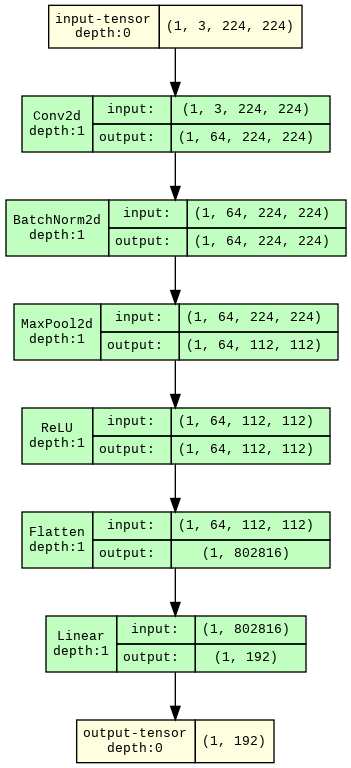
\includegraphics[width=0.247\textwidth]{./assets/CustomCNN_visualization.png}
    \captionsetup{justification=centering}
    \caption{Custom CNN network used to experiment with hyper-parameters}
    \label{fig:custom_cnn_chart}
  \end{center}
\end{figure}


\subsection{Learning Rate}

The learning rate is a hyper-parameter that controls the amount of optimization done during the training phase.
It is a scalar value that controls how much the optimizers can change the model's weights.
% \subsection{Weight Decay}

% Test the impact of weight decay on model generalization by varying values (e.g., 1e-4, 1e-5).

\subsection{Optimizer}

Try different optimizers (e.g., SGD, Adam, RMSprop) and observe their effects on convergence.

\subsection{Batch Size}

Evaluate performance with various batch sizes to find a balance between training speed and memory usage.

\subsection{Number of Epochs}

Experiment with the number of training epochs to prevent underfitting or overfitting.

\subsection{Learning Rate Schedulers}

Implement schedulers like ReduceLROnPlateau or Cyclical Learning Rates to dynamically adjust the learning rate based on model performance.

\subsection{Dropout Rate}

Introduce dropout layers and experiment with dropout rates to prevent overfitting.

\subsection{Activation Functions}

Try different activation functions (e.g., ReLU, Leaky ReLU, Sigmoid) and assess their impact on convergence.

\subsection{Data Augmentation}

Explore various data augmentation techniques (e.g., rotation, flipping, scaling) to improve model robustness.


\section{Deep model architectures}
\label{sec:deep_model_arch}


\section{Conclusion}
\label{sec:conclusion}


%%%%%%%%% REFERENCES
{\small
  \bibliographystyle{ieee_fullname}
  \bibliography{egbib}
}

\end{document}
